Ein Plattenleger hat Platten verschiedener Farben zur Verfügung, um
den Boden eines kleinen Raums auszulegen, der mit $3\times 4$ Platten
gerade abgedeckt werden kann.
\begin{teilaufgaben}
\item
Wieviele verschiedene Farbmuster sind möglich, wenn die drei
Farben Weiss, Grau und Schwarz zur Verfügung stehen?
\item
Wieviele Farbmuster sind möglich, wenn jede zweite Platte 
grau sein muss?
\item
Auf wieviele Arten kann der Raum mit 5 schwarzen und 7 weissen 
Platten ausgelegt werden?
\item
Auf wieviele Arten kann der Raum mit 5 schwarzen, 4 grauen
und 3 weissen Platten ausgelegt werden?
\item
Auf wieviele Arten kann der Boden gelegt werden, wenn je drei Platten
von vier verschiedenen Farben zur Verfügung stehen?
\item
Auf wieviele Arten kann der Boden mit zwei Farben gelegt
werden, wenn gegenüberliegende Ecken die gleich, benachbarte 
Ecken verschiedene Farben haben müssen?
\end{teilaufgaben}

\begin{loesung}
\begin{teilaufgaben}
\item
Dies ist ein Perlenkettenproblem, es muss 12 Mal eine Auswahl
zwischen drei Farben getroffen werden.
Dies ist auf $3^{12}=531441$ Arten möglich.
\item
Sechs der Platten (die jeweils zweiten, siehe auch die Diskussion)
sind bereits festgelegt, das Auswahlproblem ist also beschränkt
auf 6 Platten.
Dafür bleiben $3^6=729$ Möglichkeiten.
\item
Dies ist ein Auswahlproblem, die gesuchte Anzahl wird vom
Binomialkoeffizienten geliefert.
Sie ist
\[
\binom{12}{5}
=
\frac{12\cdot 11\cdot 10\cdot 9\cdot 8}{5!}
=
792.
\]
\item
Zunächst müssen die Plätze für die 5 schwarzen Platten gewählt werden,
dies ist gemäss der vorangegangenen Teilaufgabe auf $\binom{12}{5}$
Arten möglich.
Von den verbleibenden 7 Plätzen müssen 4 für die grauen Platten gewählt
werden, was einen weiteren Faktor $\binom{7}{4}$ liefert.
Die Anzahl ist daher
\[
\binom{12}{5}\binom{7}{4}
=
792\cdot 35
=
27720.
\]
Man kann die Anzahl auch mit Fakultäten ausdrücken:
\[
\frac{12!}{5!\cdot 7!}\frac{7!}{4!\cdot 3!}
=
\frac{12!}{5!\cdot 4!\cdot 3!}
=
\binom{12}{5,4,3}.
\]
\item
Nach der gleichen Vorgehensweise von wie in der vorangegangenen
Teilaufgabe müssen nacheinander die Plätze für die verschiedenfarbigen
Platten reserviert werden.
Dies führt auf die Anzahl
\begin{align*}
\binom{12}{3}
\binom{9}{3}
\binom{6}{3}
&=
220\cdot 84\cdot 20
=
369600
\intertext{oder alternativ mit Fakultäten}
&=
\frac{12!}{3!\cdot 9!}
\frac{9!}{3!\cdot 6!}
\frac{6!}{3!\cdot 3!}
=
\frac{12!}{3!\cdot 3!\cdot 3!\cdot 3!}
=
\frac{12!}{3!^4}
=
369600.
\end{align*}
\item
Durch die Wahl einer von zwei Farben in einer Ecke sind alle anderen
Ecken bereits festgelegt.
Es bleiben also nur noch 8 Platten zu wählen, was auf $2^8$ möglich
ist.
Die Gesamtzahl ergibt sich als Produkt $2\cdot 2^8=2^9=512$.
\qedhere
\end{teilaufgaben}
\end{loesung}

\begin{diskussion}
Die Aufgabe zeigt, dass das normalerweise mit dem Binomalkoeffzienten
gelöste Auswahlproblem auf mehr als zwei Farben verallgemeinert werden
kann.
Wenn Plätze für jeweils $k_i$ Farben $i=1,\dots,l$ gewählt werden
müssen, wobei $n=k_1+\dots+k_l$, dann ist dies auf
\begin{equation}
\binom{n}{k_1,\dots,k_l}
=
\frac{n!}{k_1!\cdot\ldots\cdot k_l!}
\label{10000030:multi}
\end{equation}
Arten möglich.
Diese Verallgemeinerung des Binomialkoeffizienten in
\eqref{10000030:multi} heisst der {\em Multinomialkoeffizient}.

In der Teilaufgabe b) kann die Formulierung ``jede zweite Platte''
Verwirrung stiften.
Wenn man sich die Platten nummeriert vorstellt, dann bedeutet die
Formulierung strikt interpretiert, dass die gerade nummerierten Platten
grau sein müssen.
Man kann aber auch argumentieren, dass die Formulierung als ``die
Platten haben abwechselnd eine beliebige Farbe oder sind grau'',
dann gibt es mehr Möglichkeiten.
Viele haben geschlossen, dass es zwei Möglichkeiten gibt, nämlich die
gerade nummerierten und die ungerade nummerierten Platten.
Dies ist aber nur eine mögliche Interpretation.
Es gibt aber weitere Möglichkeiten, je nachdem in welcher Richtung
(horizontal oder vertikal) man mit dem abzählen beginnt, nämlich
\begin{center}
\def\feld#1#2{
	\fill[color=gray] ({(#1)*0.5},{(#2)*0.5}) rectangle ++ (0.5,0.5);
}
\def\rechteck{
	\foreach \x in {0,...,4}{
		\draw ({0.5*\x},0) -- ++(0,{3*0.5});
	}
	\foreach \y in {0,...,3}{
		\draw (0,{0.5*\y}) -- ++({4*0.5},0);
	}
}
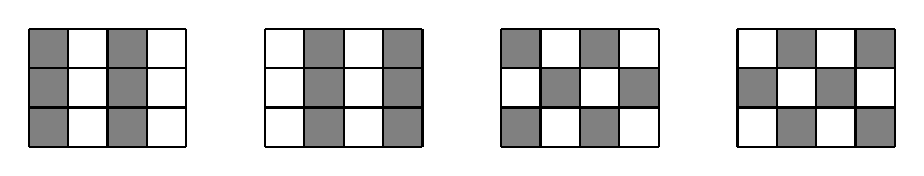
\begin{tikzpicture}[>=latex,thick]

\begin{scope}
\feld{0}{2}
\feld{2}{2}
\feld{0}{1}
\feld{2}{1}
\feld{0}{0}
\feld{2}{0}
\rechteck
\end{scope}

\begin{scope}[xshift=3cm]
\feld{1}{2}
\feld{3}{2}
\feld{1}{1}
\feld{3}{1}
\feld{1}{0}
\feld{3}{0}
\rechteck
\end{scope}

\begin{scope}[xshift=6cm]
\feld{0}{2}
\feld{0}{0}
\feld{1}{1}
\feld{2}{2}
\feld{2}{0}
\feld{3}{1}
\rechteck
\end{scope}

\begin{scope}[xshift=9cm]
\feld{0}{1}
\feld{1}{2}
\feld{1}{0}
\feld{2}{1}
\feld{3}{2}
\feld{3}{0}
\rechteck
\end{scope}

\end{tikzpicture}
\end{center}
In dieser Interpretation gibt es aber noch eine weitere Komplikation:
die Möglichkeit, nur graue Platten zu verwenden, wird mehrfach 
gezählt.
\end{diskussion}


\begin{bewertung}
Jede Teilaufgabe ({\bf A} bis {\bf F}) 1 Punkt.
\end{bewertung}
